\documentclass[11pt]{article}
\usepackage[textwidth=18.0cm, textheight=23.0cm, top=2.0cm]{geometry}
\usepackage{pst-all}
\usepackage{amssymb}
\usepackage{tikz}
\usepackage{underscore}\begin{document}
\pagestyle{empty}


ClassName: \underline{\textbf{Class_10.2bp-20}}
\par
BinSize: \underline{\textbf{100 × 100}}
\par
ReduceSize: \underline{\textbf{100 × 100}}
\par
TypeNum: \underline{\textbf{60}}
\par
Num: \underline{\textbf{60}}
\par
OutS: \underline{\textbf{120000}}
\par
InS: \underline{\textbf{103184}}
\par
Rate: \underline{\textbf{0.860}}
\par
UB: \underline{\textbf{12}}
\par
LB0: \underline{\textbf{11}}
\par
LB: \underline{\textbf{12}}
\par
LBWithCut: \underline{\textbf{12}}
\par
NodeCut: \underline{\textbf{0}}
\par
ExtendedNodeCnt: \underline{\textbf{1}}
\par
GenNodeCnt: \underline{\textbf{1}}
\par
PrimalNode: \underline{\textbf{0}}
\par
ColumnCount: \underline{\textbf{49}}
\par
TotalCutCount: \underline{\textbf{0}}
\par
RootCutCount: \underline{\textbf{0}}
\par
LPSolverCnt: \underline{\textbf{38}}
\par
PricingSolverCnt: \underline{\textbf{38}}
\par
BranchAndBoundNum: \underline{\textbf{1}}
\par
isOpt: \underline{\textbf{false}}
\par
TimeOnInitSolution: \underline{\textbf{600.000 s}}
\par
TimeOnPrimal: \underline{\textbf{0.000 s}}
\par
TimeOnPricing: \underline{\textbf{2999.666 s}}
\par
TimeOnRmp: \underline{\textbf{0.079 s}}
\par
TotalTime: \underline{\textbf{3600.011 s}}
\par
\newpage


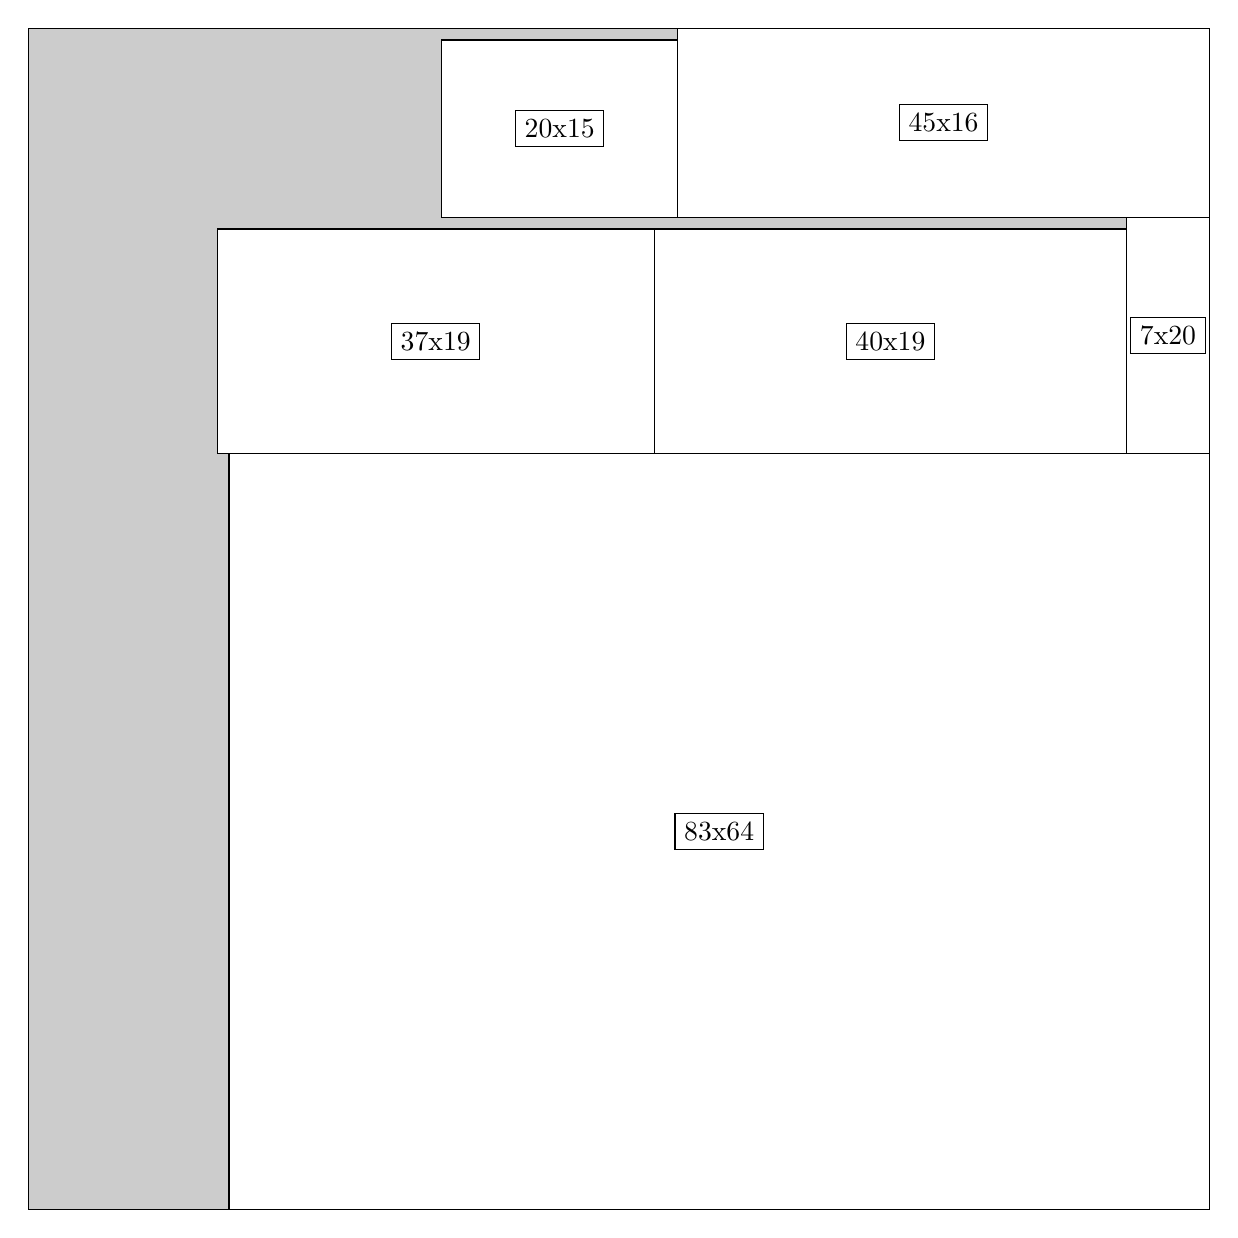
\begin{tikzpicture}[shorten >=1pt,scale=1.0,every node/.style={scale=1.0},->]
\tikzstyle{vertex}=[circle,fill=black!25,minimum size=14pt,inner sep=0pt]
\filldraw[fill=gray!40!white, draw=black] (0,0) rectangle (15.0,15.0);
\foreach \name/\x/\y/\w/\h in {83x64/2.55/0.0/12.45/9.6,7x20/13.95/9.6/1.05/3.0,40x19/7.949999999999999/9.6/6.0/2.85,37x19/2.4/9.6/5.55/2.85,45x16/8.25/12.6/6.75/2.4,20x15/5.25/12.6/3.0/2.25}
\filldraw[fill=white!40!white, draw=black] (\x,\y) rectangle node[draw] (\name) {\name} ++(\w,\h);
\end{tikzpicture}


w =83 , h =64 , x =17 , y =0 , v =5312
\par
w =7 , h =20 , x =93 , y =64 , v =140
\par
w =40 , h =19 , x =53 , y =64 , v =760
\par
w =37 , h =19 , x =16 , y =64 , v =703
\par
w =45 , h =16 , x =55 , y =84 , v =720
\par
w =20 , h =15 , x =35 , y =84 , v =300
\par
\newpage


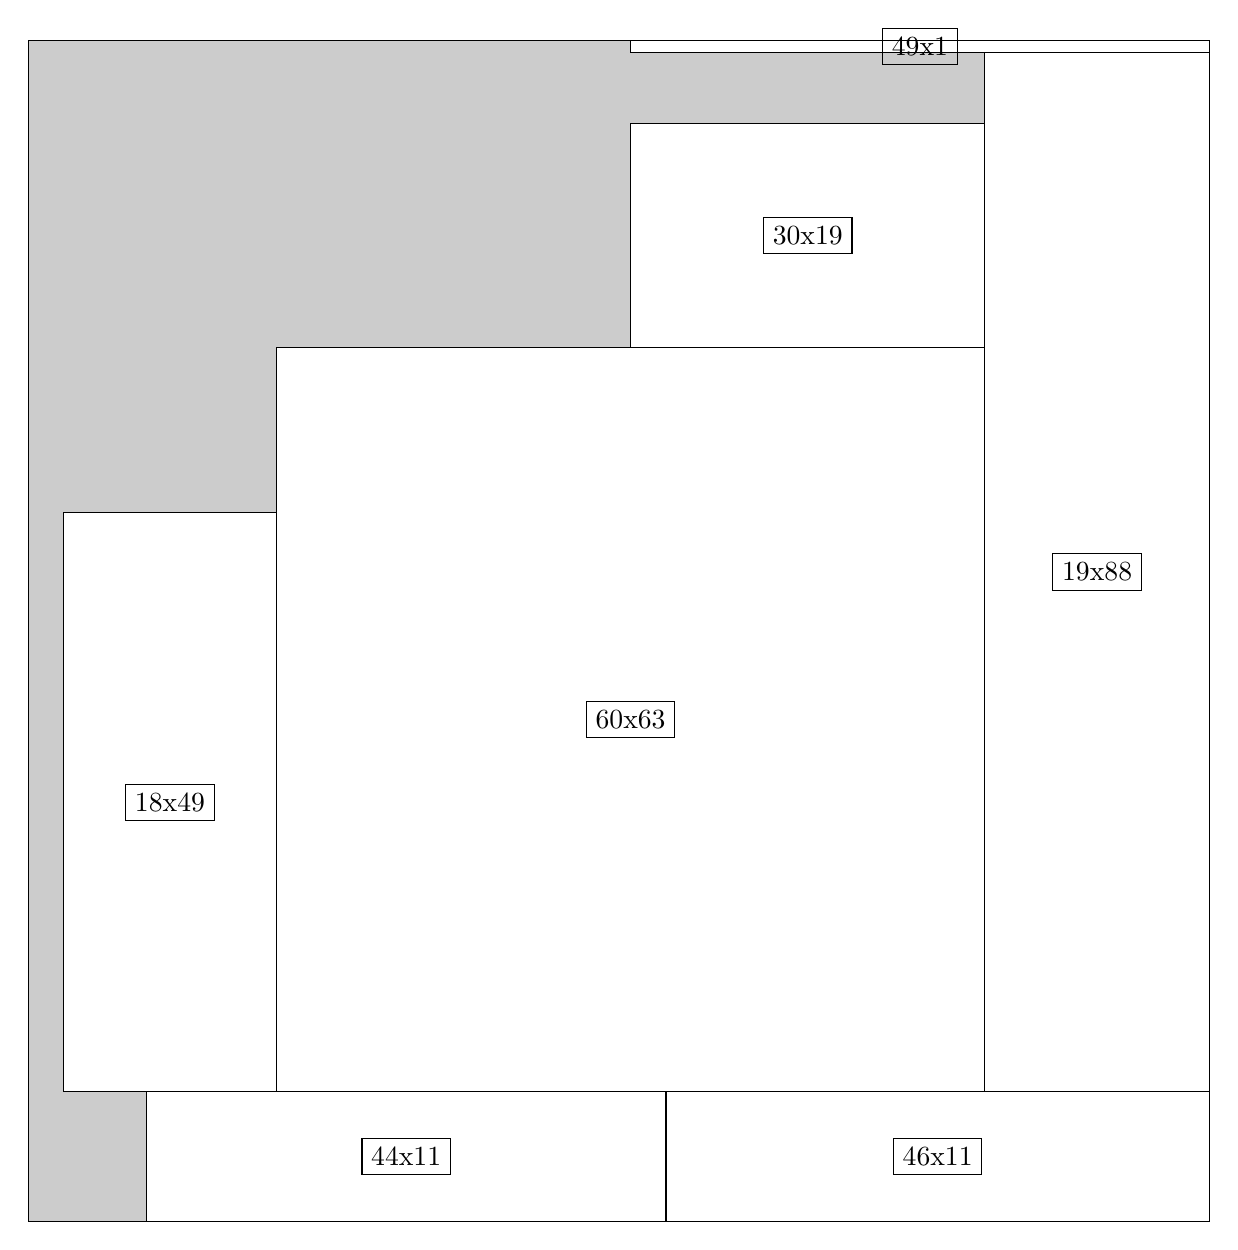
\begin{tikzpicture}[shorten >=1pt,scale=1.0,every node/.style={scale=1.0},->]
\tikzstyle{vertex}=[circle,fill=black!25,minimum size=14pt,inner sep=0pt]
\filldraw[fill=gray!40!white, draw=black] (0,0) rectangle (15.0,15.0);
\foreach \name/\x/\y/\w/\h in {46x11/8.1/0.0/6.8999999999999995/1.65,44x11/1.5/0.0/6.6/1.65,19x88/12.15/1.65/2.85/13.2,60x63/3.15/1.65/9.0/9.45,18x49/0.44999999999999996/1.65/2.6999999999999997/7.35,30x19/7.6499999999999995/11.1/4.5/2.85,49x1/7.6499999999999995/14.85/7.35/0.15}
\filldraw[fill=white!40!white, draw=black] (\x,\y) rectangle node[draw] (\name) {\name} ++(\w,\h);
\end{tikzpicture}


w =46 , h =11 , x =54 , y =0 , v =506
\par
w =44 , h =11 , x =10 , y =0 , v =484
\par
w =19 , h =88 , x =81 , y =11 , v =1672
\par
w =60 , h =63 , x =21 , y =11 , v =3780
\par
w =18 , h =49 , x =3 , y =11 , v =882
\par
w =30 , h =19 , x =51 , y =74 , v =570
\par
w =49 , h =1 , x =51 , y =99 , v =49
\par
\newpage


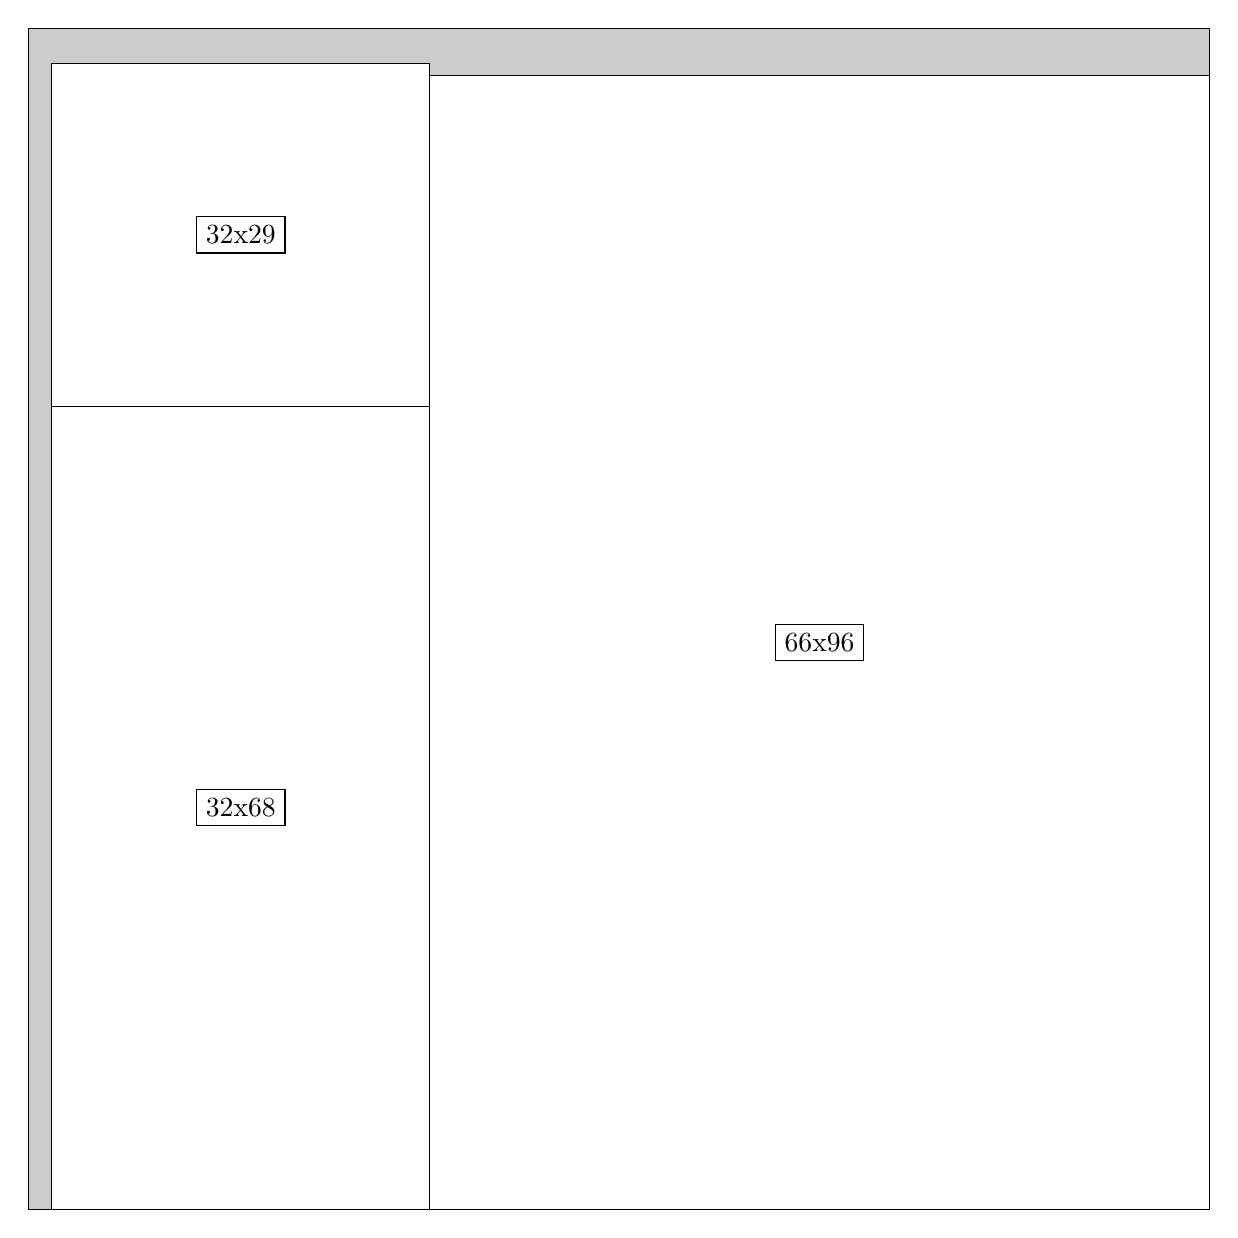
\begin{tikzpicture}[shorten >=1pt,scale=1.0,every node/.style={scale=1.0},->]
\tikzstyle{vertex}=[circle,fill=black!25,minimum size=14pt,inner sep=0pt]
\filldraw[fill=gray!40!white, draw=black] (0,0) rectangle (15.0,15.0);
\foreach \name/\x/\y/\w/\h in {66x96/5.1/0.0/9.9/14.399999999999999,32x68/0.3/0.0/4.8/10.2,32x29/0.3/10.2/4.8/4.35}
\filldraw[fill=white!40!white, draw=black] (\x,\y) rectangle node[draw] (\name) {\name} ++(\w,\h);
\end{tikzpicture}


w =66 , h =96 , x =34 , y =0 , v =6336
\par
w =32 , h =68 , x =2 , y =0 , v =2176
\par
w =32 , h =29 , x =2 , y =68 , v =928
\par
\newpage


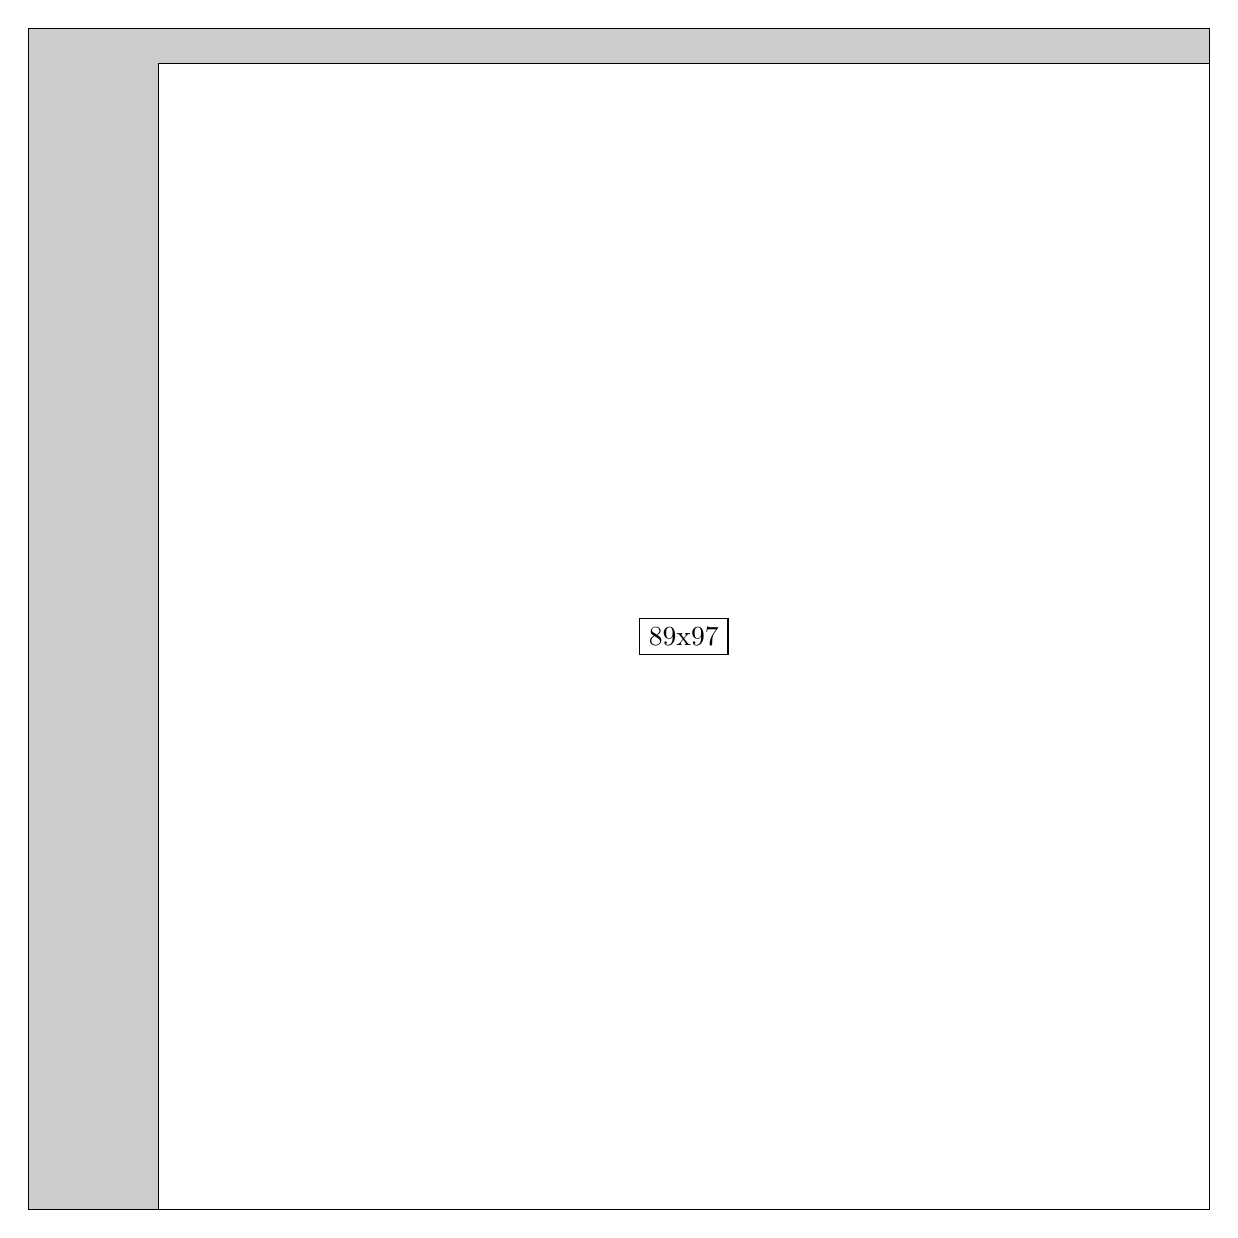
\begin{tikzpicture}[shorten >=1pt,scale=1.0,every node/.style={scale=1.0},->]
\tikzstyle{vertex}=[circle,fill=black!25,minimum size=14pt,inner sep=0pt]
\filldraw[fill=gray!40!white, draw=black] (0,0) rectangle (15.0,15.0);
\foreach \name/\x/\y/\w/\h in {89x97/1.65/0.0/13.35/14.549999999999999}
\filldraw[fill=white!40!white, draw=black] (\x,\y) rectangle node[draw] (\name) {\name} ++(\w,\h);
\end{tikzpicture}


w =89 , h =97 , x =11 , y =0 , v =8633
\par
\newpage


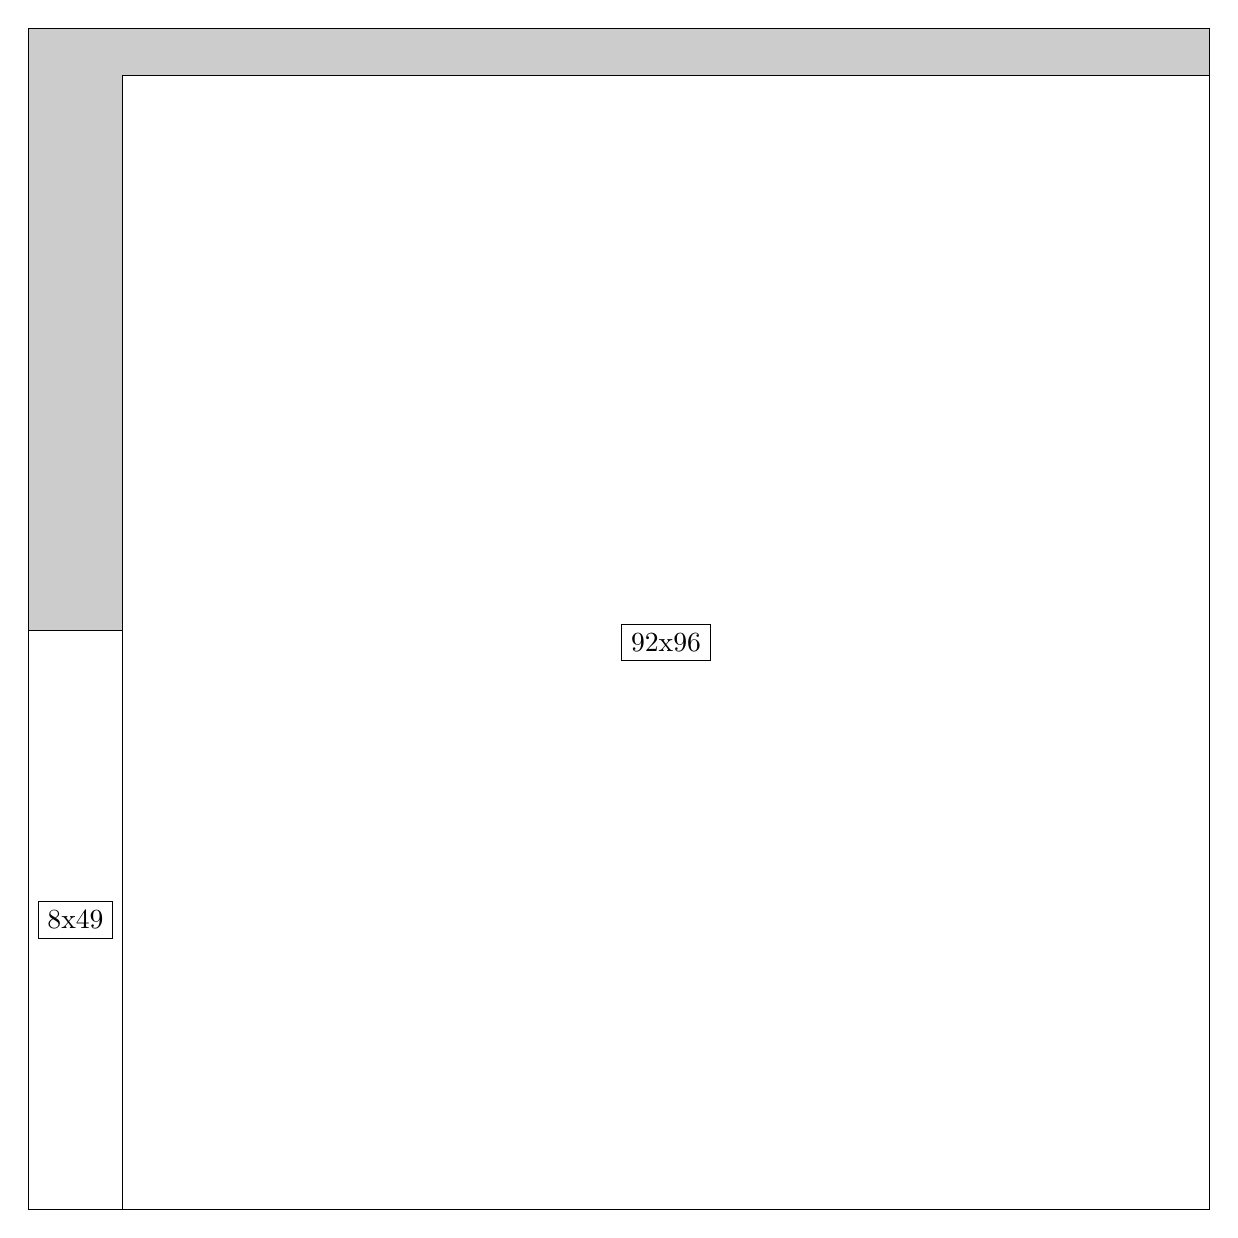
\begin{tikzpicture}[shorten >=1pt,scale=1.0,every node/.style={scale=1.0},->]
\tikzstyle{vertex}=[circle,fill=black!25,minimum size=14pt,inner sep=0pt]
\filldraw[fill=gray!40!white, draw=black] (0,0) rectangle (15.0,15.0);
\foreach \name/\x/\y/\w/\h in {92x96/1.2/0.0/13.799999999999999/14.399999999999999,8x49/0.0/0.0/1.2/7.35}
\filldraw[fill=white!40!white, draw=black] (\x,\y) rectangle node[draw] (\name) {\name} ++(\w,\h);
\end{tikzpicture}


w =92 , h =96 , x =8 , y =0 , v =8832
\par
w =8 , h =49 , x =0 , y =0 , v =392
\par
\newpage


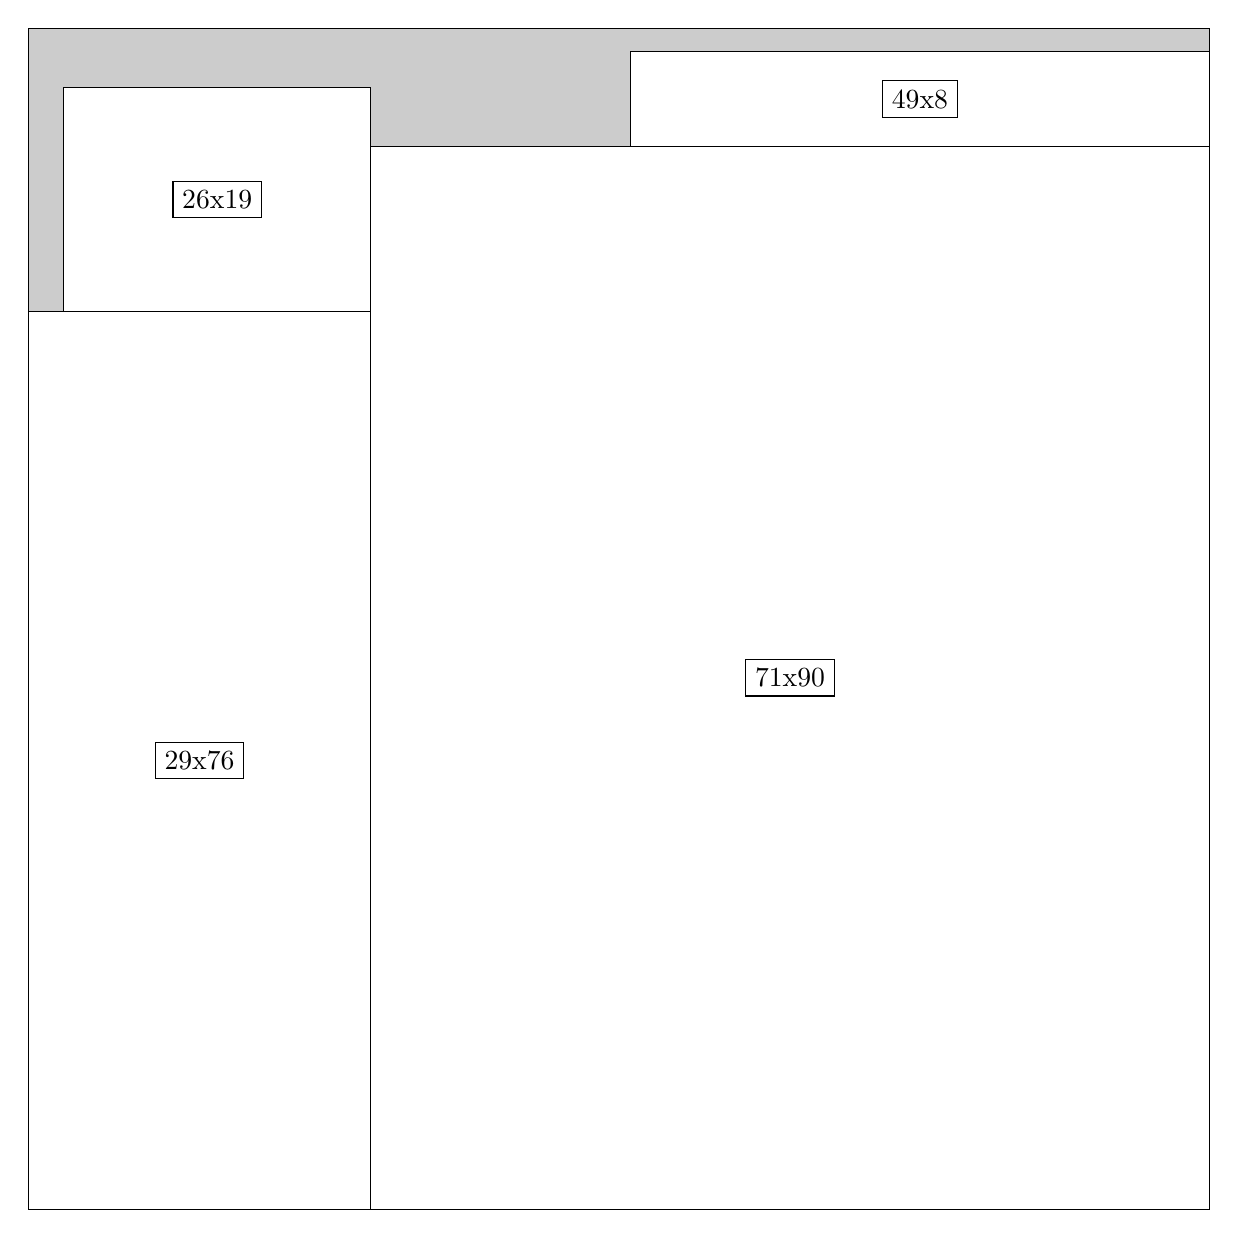
\begin{tikzpicture}[shorten >=1pt,scale=1.0,every node/.style={scale=1.0},->]
\tikzstyle{vertex}=[circle,fill=black!25,minimum size=14pt,inner sep=0pt]
\filldraw[fill=gray!40!white, draw=black] (0,0) rectangle (15.0,15.0);
\foreach \name/\x/\y/\w/\h in {71x90/4.35/0.0/10.65/13.5,49x8/7.6499999999999995/13.5/7.35/1.2,29x76/0.0/0.0/4.35/11.4,26x19/0.44999999999999996/11.4/3.9/2.85}
\filldraw[fill=white!40!white, draw=black] (\x,\y) rectangle node[draw] (\name) {\name} ++(\w,\h);
\end{tikzpicture}


w =71 , h =90 , x =29 , y =0 , v =6390
\par
w =49 , h =8 , x =51 , y =90 , v =392
\par
w =29 , h =76 , x =0 , y =0 , v =2204
\par
w =26 , h =19 , x =3 , y =76 , v =494
\par
\newpage


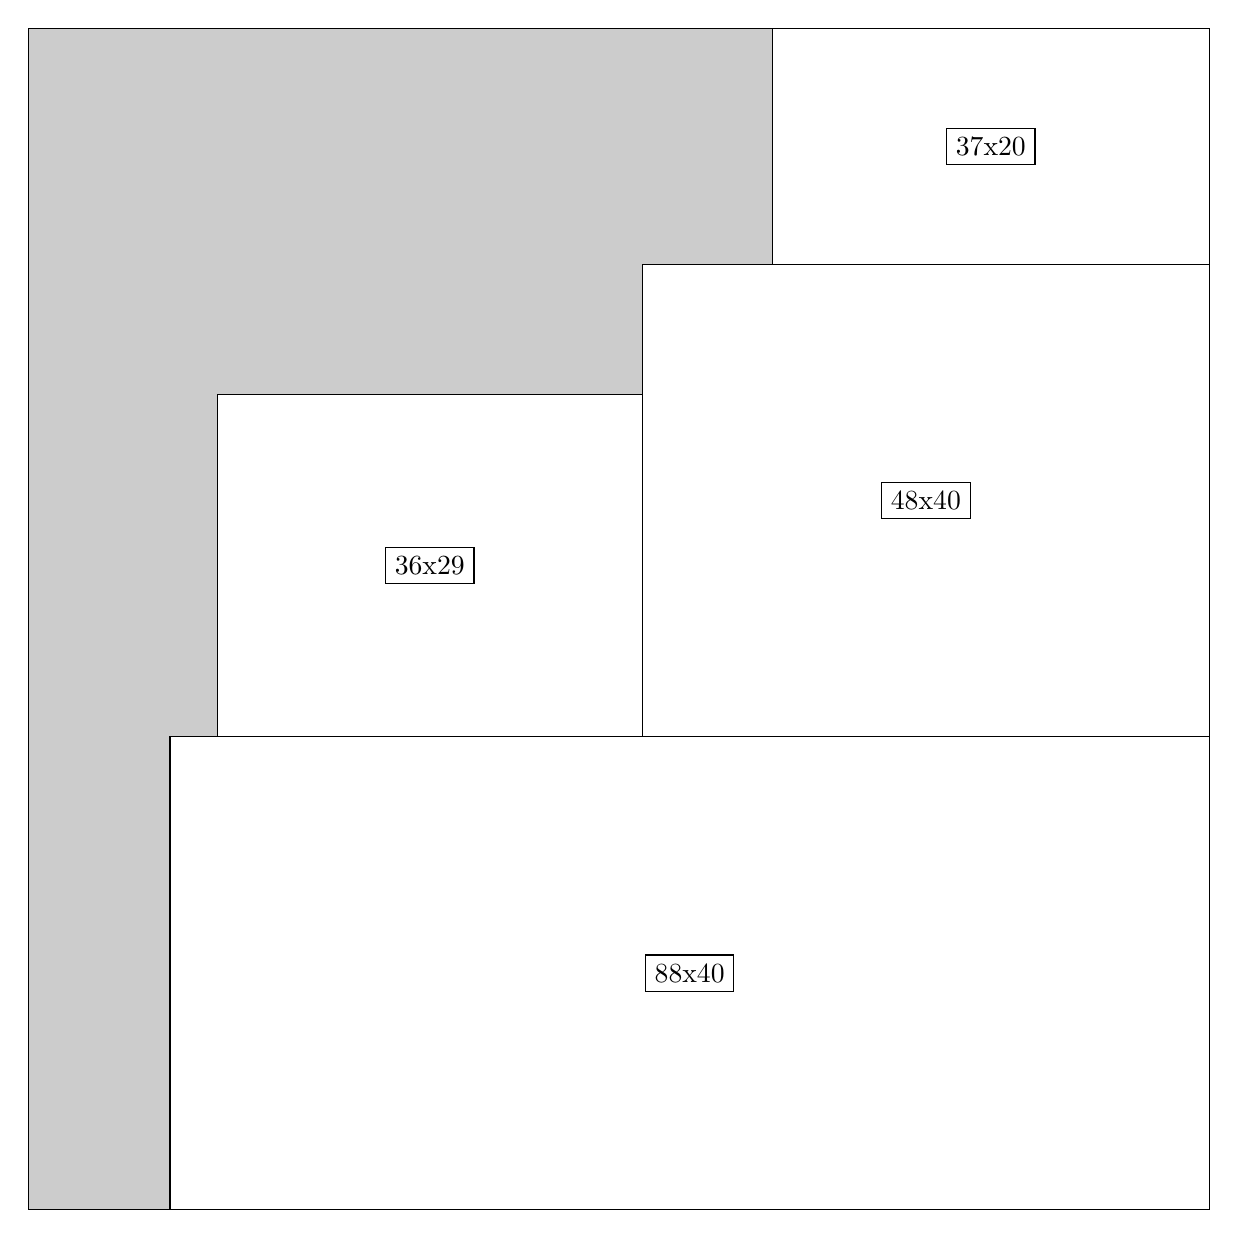
\begin{tikzpicture}[shorten >=1pt,scale=1.0,every node/.style={scale=1.0},->]
\tikzstyle{vertex}=[circle,fill=black!25,minimum size=14pt,inner sep=0pt]
\filldraw[fill=gray!40!white, draw=black] (0,0) rectangle (15.0,15.0);
\foreach \name/\x/\y/\w/\h in {88x40/1.7999999999999998/0.0/13.2/6.0,48x40/7.8/6.0/7.199999999999999/6.0,37x20/9.45/12.0/5.55/3.0,36x29/2.4/6.0/5.3999999999999995/4.35}
\filldraw[fill=white!40!white, draw=black] (\x,\y) rectangle node[draw] (\name) {\name} ++(\w,\h);
\end{tikzpicture}


w =88 , h =40 , x =12 , y =0 , v =3520
\par
w =48 , h =40 , x =52 , y =40 , v =1920
\par
w =37 , h =20 , x =63 , y =80 , v =740
\par
w =36 , h =29 , x =16 , y =40 , v =1044
\par
\newpage


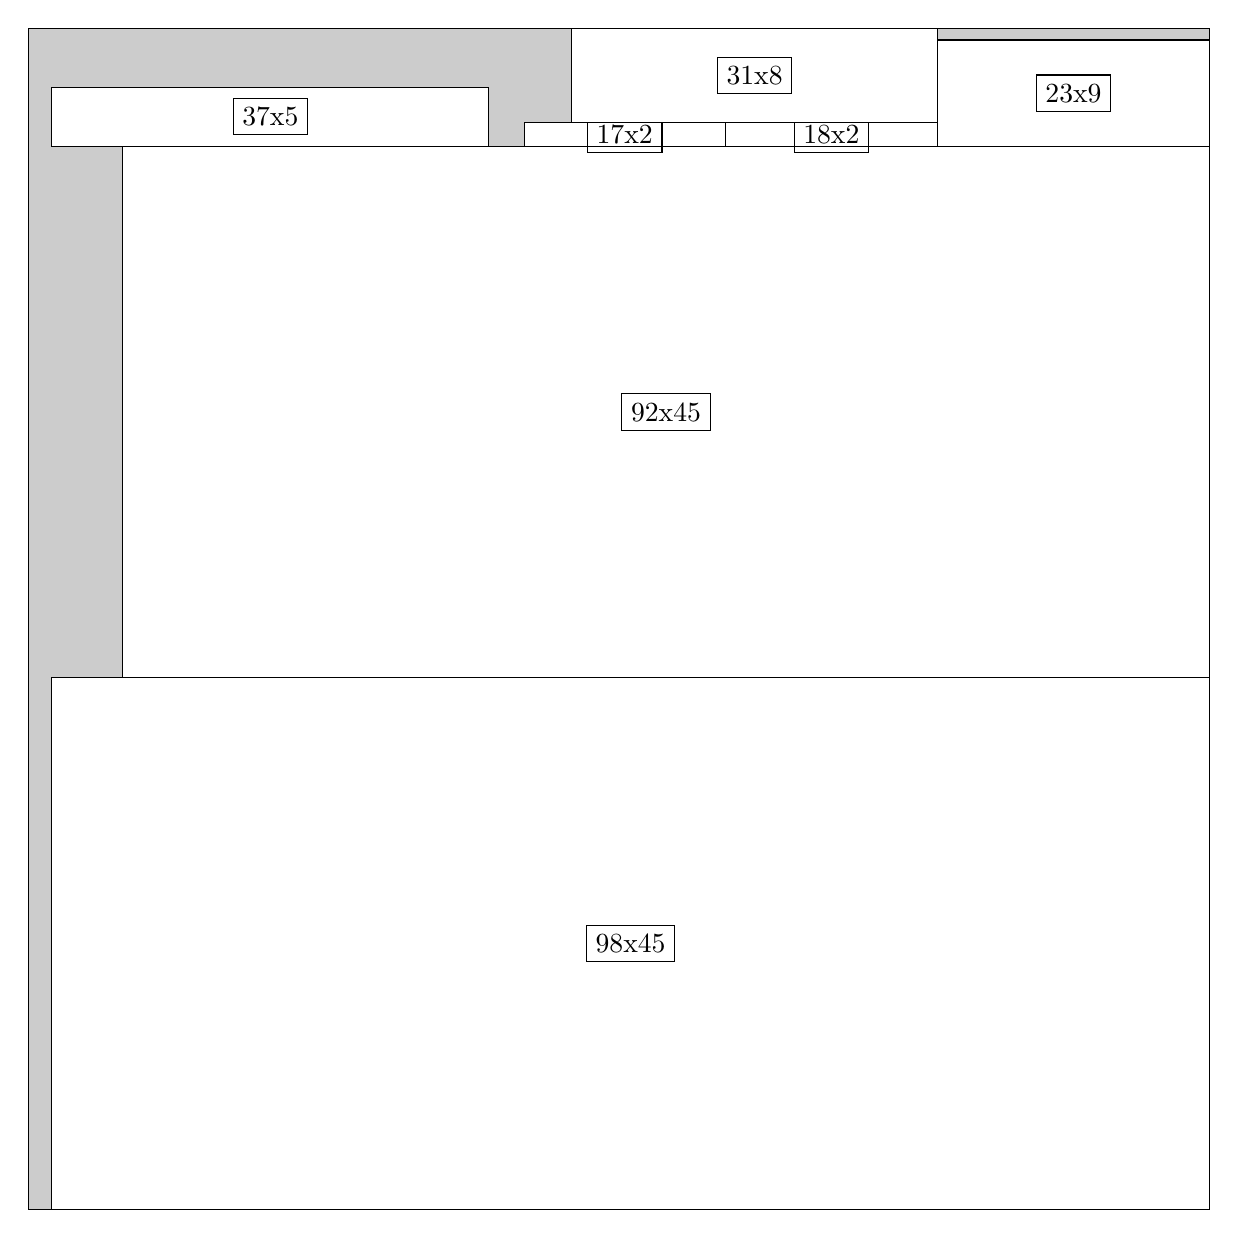
\begin{tikzpicture}[shorten >=1pt,scale=1.0,every node/.style={scale=1.0},->]
\tikzstyle{vertex}=[circle,fill=black!25,minimum size=14pt,inner sep=0pt]
\filldraw[fill=gray!40!white, draw=black] (0,0) rectangle (15.0,15.0);
\foreach \name/\x/\y/\w/\h in {98x45/0.3/0.0/14.7/6.75,92x45/1.2/6.75/13.799999999999999/6.75,23x9/11.549999999999999/13.5/3.4499999999999997/1.3499999999999999,18x2/8.85/13.5/2.6999999999999997/0.3,17x2/6.3/13.5/2.55/0.3,31x8/6.8999999999999995/13.799999999999999/4.6499999999999995/1.2,37x5/0.3/13.5/5.55/0.75}
\filldraw[fill=white!40!white, draw=black] (\x,\y) rectangle node[draw] (\name) {\name} ++(\w,\h);
\end{tikzpicture}


w =98 , h =45 , x =2 , y =0 , v =4410
\par
w =92 , h =45 , x =8 , y =45 , v =4140
\par
w =23 , h =9 , x =77 , y =90 , v =207
\par
w =18 , h =2 , x =59 , y =90 , v =36
\par
w =17 , h =2 , x =42 , y =90 , v =34
\par
w =31 , h =8 , x =46 , y =92 , v =248
\par
w =37 , h =5 , x =2 , y =90 , v =185
\par
\newpage


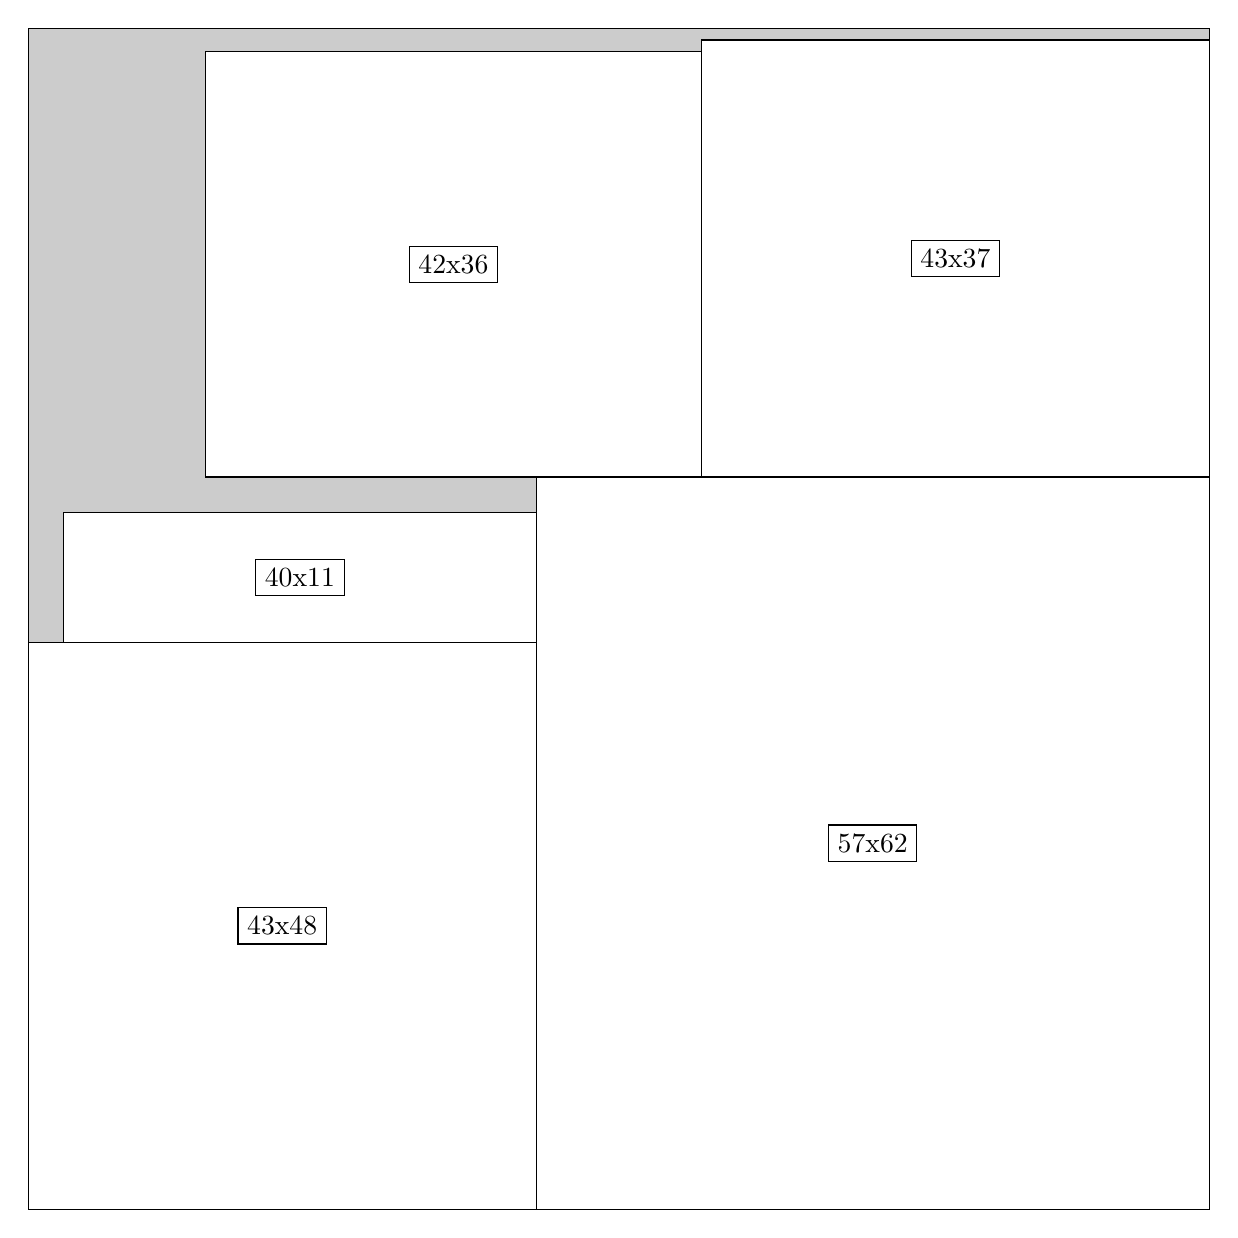
\begin{tikzpicture}[shorten >=1pt,scale=1.0,every node/.style={scale=1.0},->]
\tikzstyle{vertex}=[circle,fill=black!25,minimum size=14pt,inner sep=0pt]
\filldraw[fill=gray!40!white, draw=black] (0,0) rectangle (15.0,15.0);
\foreach \name/\x/\y/\w/\h in {57x62/6.45/0.0/8.549999999999999/9.299999999999999,43x48/0.0/0.0/6.45/7.199999999999999,40x11/0.44999999999999996/7.199999999999999/6.0/1.65,43x37/8.549999999999999/9.299999999999999/6.45/5.55,42x36/2.25/9.299999999999999/6.3/5.3999999999999995}
\filldraw[fill=white!40!white, draw=black] (\x,\y) rectangle node[draw] (\name) {\name} ++(\w,\h);
\end{tikzpicture}


w =57 , h =62 , x =43 , y =0 , v =3534
\par
w =43 , h =48 , x =0 , y =0 , v =2064
\par
w =40 , h =11 , x =3 , y =48 , v =440
\par
w =43 , h =37 , x =57 , y =62 , v =1591
\par
w =42 , h =36 , x =15 , y =62 , v =1512
\par
\newpage


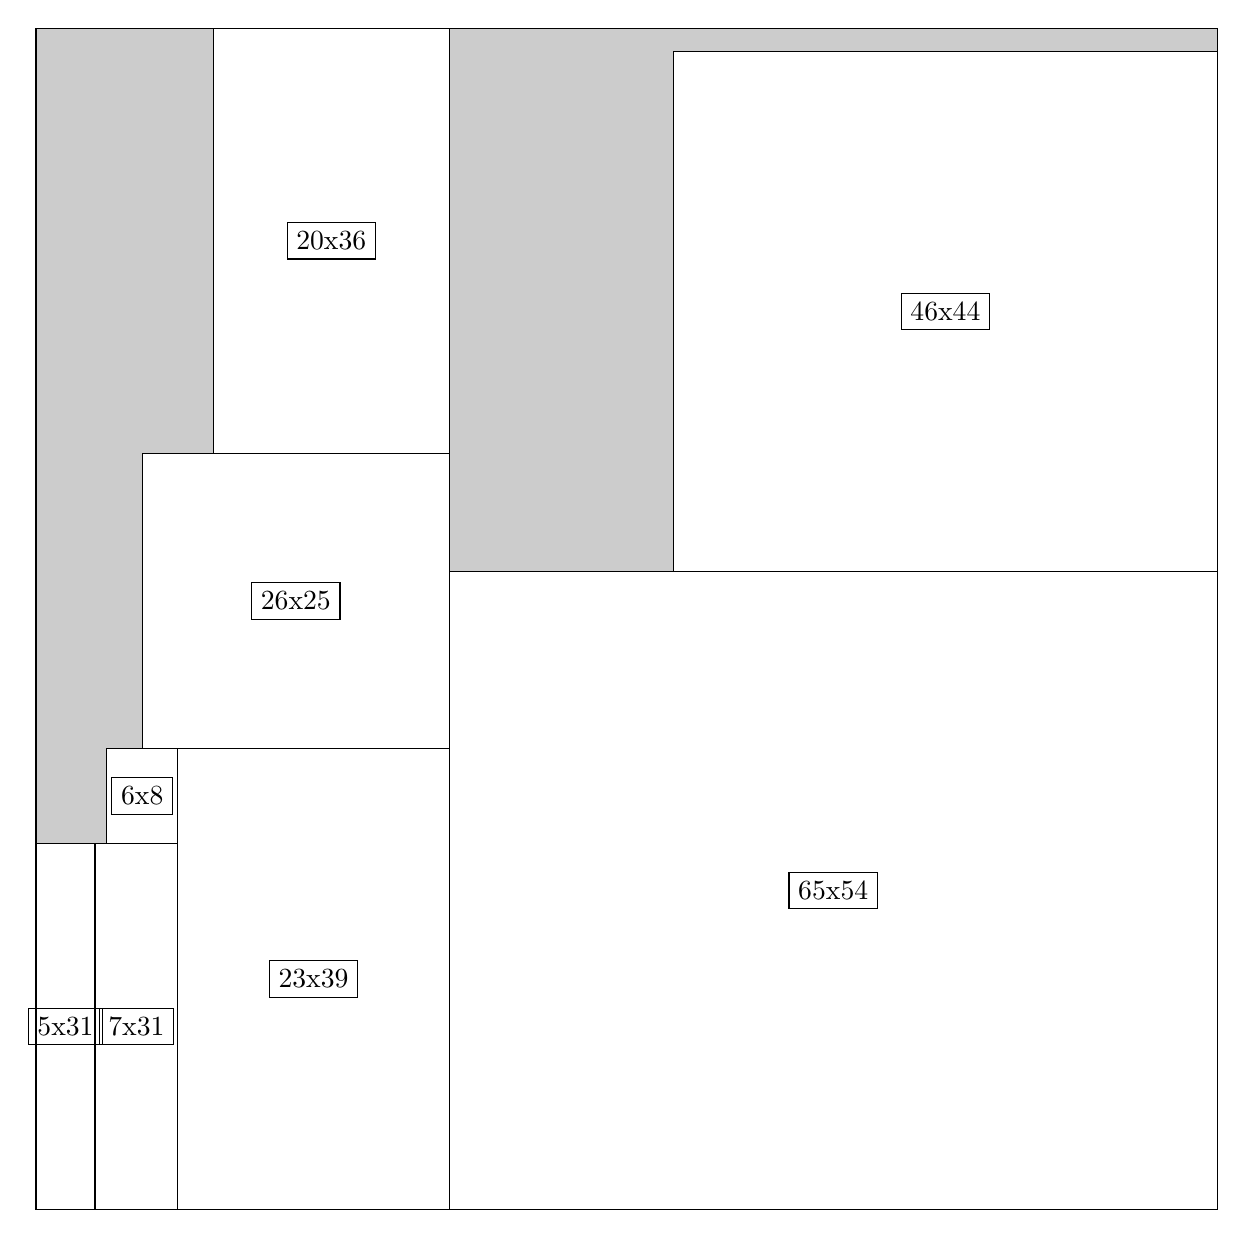
\begin{tikzpicture}[shorten >=1pt,scale=1.0,every node/.style={scale=1.0},->]
\tikzstyle{vertex}=[circle,fill=black!25,minimum size=14pt,inner sep=0pt]
\filldraw[fill=gray!40!white, draw=black] (0,0) rectangle (15.0,15.0);
\foreach \name/\x/\y/\w/\h in {65x54/5.25/0.0/9.75/8.1,46x44/8.1/8.1/6.8999999999999995/6.6,23x39/1.7999999999999998/0.0/3.4499999999999997/5.85,7x31/0.75/0.0/1.05/4.6499999999999995,6x8/0.8999999999999999/4.6499999999999995/0.8999999999999999/1.2,5x31/0.0/0.0/0.75/4.6499999999999995,26x25/1.3499999999999999/5.85/3.9/3.75,20x36/2.25/9.6/3.0/5.3999999999999995}
\filldraw[fill=white!40!white, draw=black] (\x,\y) rectangle node[draw] (\name) {\name} ++(\w,\h);
\end{tikzpicture}


w =65 , h =54 , x =35 , y =0 , v =3510
\par
w =46 , h =44 , x =54 , y =54 , v =2024
\par
w =23 , h =39 , x =12 , y =0 , v =897
\par
w =7 , h =31 , x =5 , y =0 , v =217
\par
w =6 , h =8 , x =6 , y =31 , v =48
\par
w =5 , h =31 , x =0 , y =0 , v =155
\par
w =26 , h =25 , x =9 , y =39 , v =650
\par
w =20 , h =36 , x =15 , y =64 , v =720
\par
\newpage


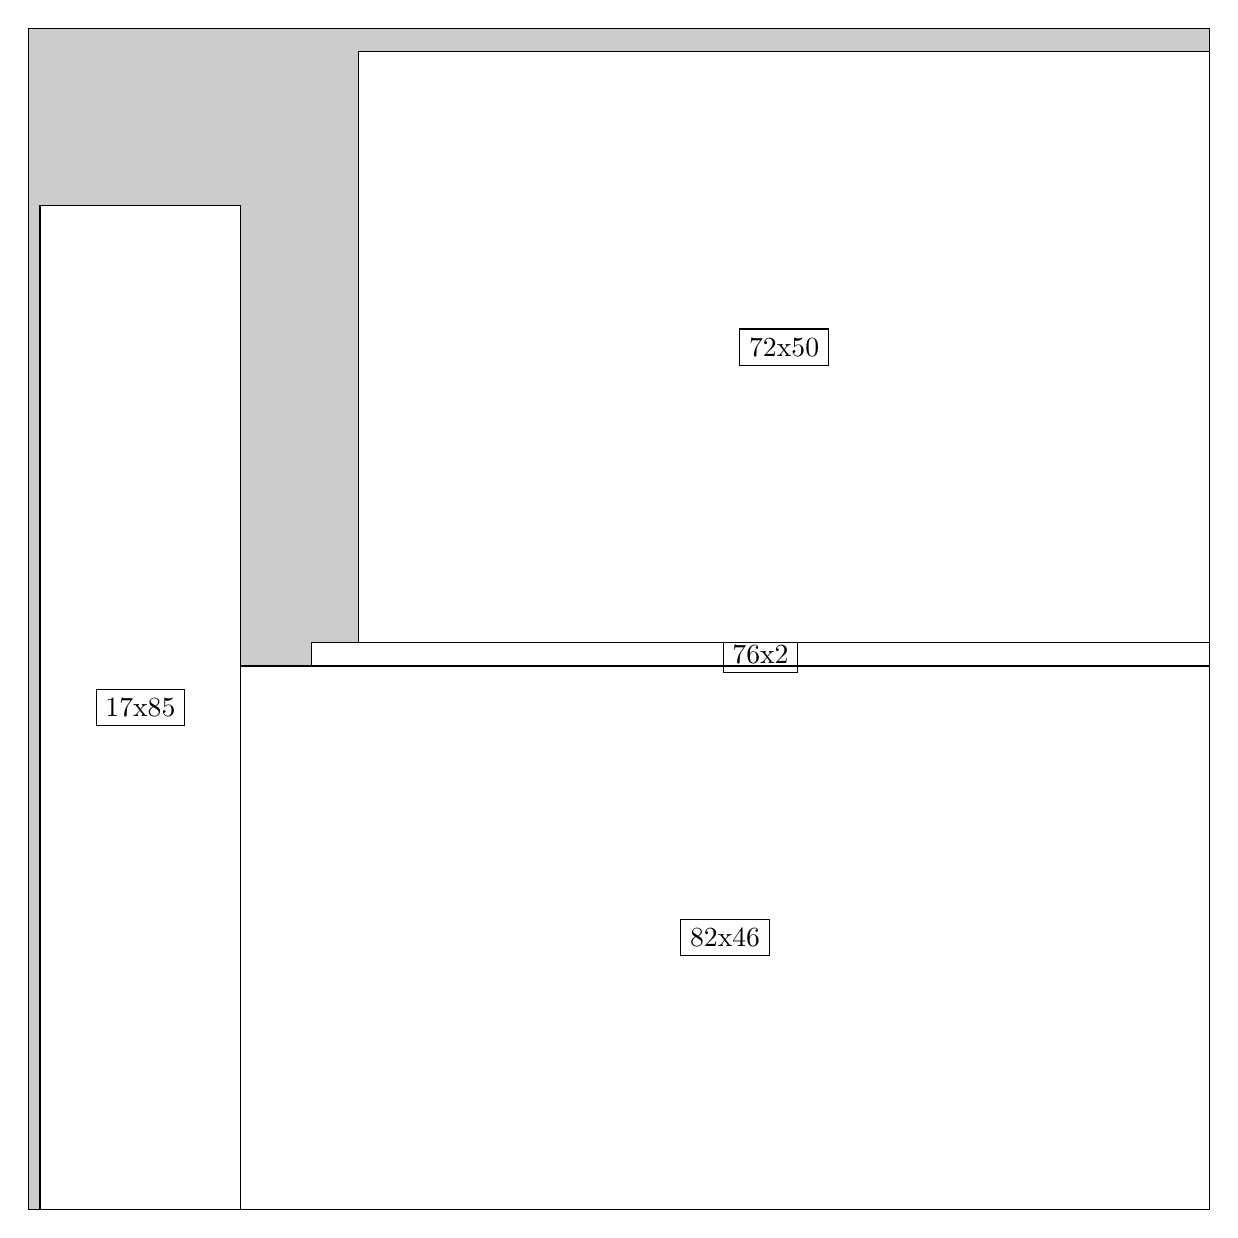
\begin{tikzpicture}[shorten >=1pt,scale=1.0,every node/.style={scale=1.0},->]
\tikzstyle{vertex}=[circle,fill=black!25,minimum size=14pt,inner sep=0pt]
\filldraw[fill=gray!40!white, draw=black] (0,0) rectangle (15.0,15.0);
\foreach \name/\x/\y/\w/\h in {82x46/2.6999999999999997/0.0/12.299999999999999/6.8999999999999995,76x2/3.5999999999999996/6.8999999999999995/11.4/0.3,72x50/4.2/7.199999999999999/10.799999999999999/7.5,17x85/0.15/0.0/2.55/12.75}
\filldraw[fill=white!40!white, draw=black] (\x,\y) rectangle node[draw] (\name) {\name} ++(\w,\h);
\end{tikzpicture}


w =82 , h =46 , x =18 , y =0 , v =3772
\par
w =76 , h =2 , x =24 , y =46 , v =152
\par
w =72 , h =50 , x =28 , y =48 , v =3600
\par
w =17 , h =85 , x =1 , y =0 , v =1445
\par
\newpage


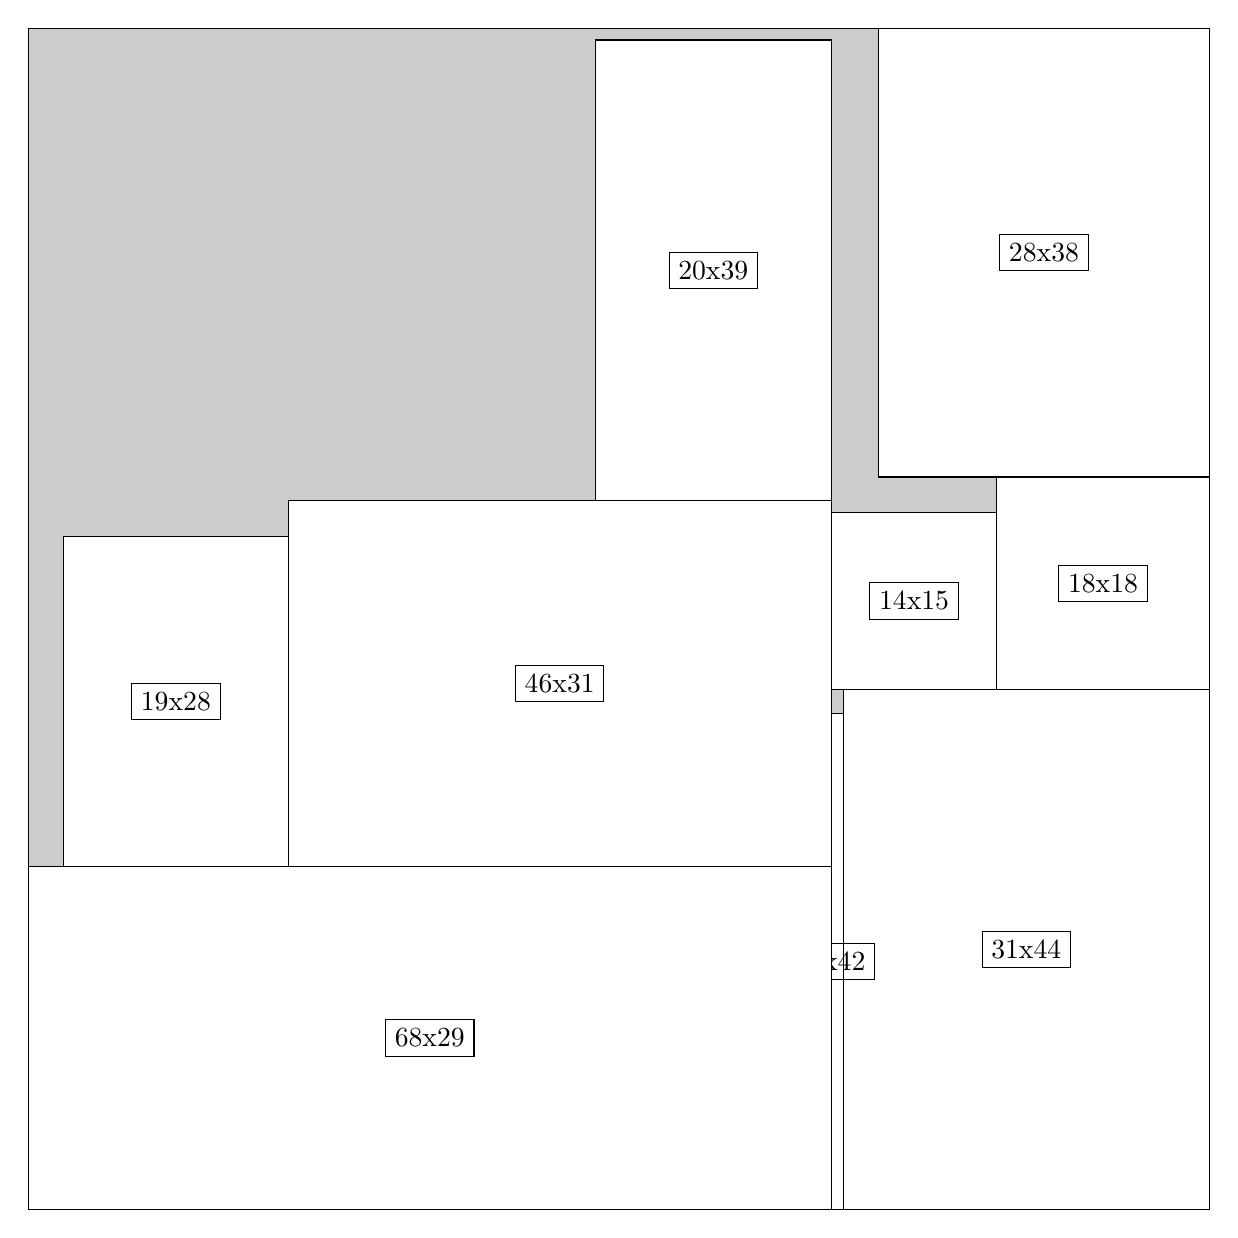
\begin{tikzpicture}[shorten >=1pt,scale=1.0,every node/.style={scale=1.0},->]
\tikzstyle{vertex}=[circle,fill=black!25,minimum size=14pt,inner sep=0pt]
\filldraw[fill=gray!40!white, draw=black] (0,0) rectangle (15.0,15.0);
\foreach \name/\x/\y/\w/\h in {31x44/10.35/0.0/4.6499999999999995/6.6,1x42/10.2/0.0/0.15/6.3,18x18/12.299999999999999/6.6/2.6999999999999997/2.6999999999999997,14x15/10.2/6.6/2.1/2.25,28x38/10.799999999999999/9.299999999999999/4.2/5.7,68x29/0.0/0.0/10.2/4.35,46x31/3.3/4.35/6.8999999999999995/4.6499999999999995,19x28/0.44999999999999996/4.35/2.85/4.2,20x39/7.199999999999999/9.0/3.0/5.85}
\filldraw[fill=white!40!white, draw=black] (\x,\y) rectangle node[draw] (\name) {\name} ++(\w,\h);
\end{tikzpicture}


w =31 , h =44 , x =69 , y =0 , v =1364
\par
w =1 , h =42 , x =68 , y =0 , v =42
\par
w =18 , h =18 , x =82 , y =44 , v =324
\par
w =14 , h =15 , x =68 , y =44 , v =210
\par
w =28 , h =38 , x =72 , y =62 , v =1064
\par
w =68 , h =29 , x =0 , y =0 , v =1972
\par
w =46 , h =31 , x =22 , y =29 , v =1426
\par
w =19 , h =28 , x =3 , y =29 , v =532
\par
w =20 , h =39 , x =48 , y =60 , v =780
\par
\newpage


\end{document}